\documentclass[9pt]{pnas-new}
% Use the lineno option to display guide line numbers if required.
% Note that the use of elements such as single-column equations
% may affect the guide line number alignment. 

% \RequirePackage[english,slovene]{babel} % when writing in slovene
\RequirePackage[slovene,english]{babel} % when writing in english

% Custom added packages
\usetikzlibrary{shapes.geometric}
\usepackage{subcaption}


\templatetype{pnasresearcharticle} % Choose template 
% {pnasresearcharticle} = Template for a two-column research article
% {pnasmathematics} = Template for a one-column mathematics article
% {pnasinvited} = Template for a PNAS invited submission

\selectlanguage{english}
%\etal{in sod.} % comment out when writing in english
%\renewcommand{\Authands}{ in } % comment out when writing in english
%\renewcommand{\Authand}{ in } % comment out when writing in english

\newcommand{\set}[1]{\ensuremath{\mathbf{#1}}}
\renewcommand{\vec}[1]{\ensuremath{\mathbf{#1}}}
\newcommand{\uvec}[1]{\ensuremath{\hat{\vec{#1}}}}
\newcommand{\const}[1]{{\ensuremath{\kappa_\mathrm{#1}}}} 

\newcommand{\num}[1]{#1}

\graphicspath{{./fig/}}

\title{Predator-Prey Simulation Using Boids Model}

% Use letters for affiliations, numbers to show equal authorship (if applicable) and to indicate the corresponding author
\author{Matija Ojo}
\author{Miha Krajnc}
\author{Marko Adžaga}
\author{Janez Kuhar}

\affil{Collective behavior course research seminar report}

% Please give the surname of the lead author for the running footer
\leadauthor{Ojo} 

\selectlanguage{english}

% Please add here a significance statement to explain the relevance of your work
\significancestatement{Collective behavior course research seminar report}{Predator-prey interactions is of significant importance in biology and nature itself. The insights gleaned from this research can offer more than a theoretical understanding; they pave the way for the design and optimization of autonomous agents capable of adaptive and context-aware behaviors. The applications range from research in biology to simulations of large amounts of boids found in computer graphics.}{Collective behavior | Boids | Simulation | Prey-Predator | Escape patterns}

\selectlanguage{english}

% Please include corresponding author, author contribution and author declaration information
%\authorcontributions{Please provide details of author contributions here.}
%\authordeclaration{Please declare any conflict of interest here.}
%\equalauthors{\textsuperscript{1}A.O.(Author One) and A.T. (Author Two) contributed equally to this work (remove if not applicable).}
%\correspondingauthor{\textsuperscript{2}To whom correspondence should be addressed. E-mail: author.two\@email.com}

% Keywords are not mandatory, but authors are strongly encouraged to provide them. If provided, please include two to five keywords, separated by the pipe symbol, e.g:
\keywords{Collective behavior | Boids | Simulation | Prey-Predator | Escape patterns } 

\begin{abstract}
The collective behaviors observed in nature, such as flocking, herding, or schooling, often serve as adaptive strategies that enhance the survival chances of individuals within a group.
Understanding these natural behaviors serves as inspiration for designing autonomous agents capable of sophisticated interactions within a simulated environment.
Our goal is to simulate prey and predator with different predator tactics (attack center, attack nearest, attack isolated, attacks from various directions, constant bearing hunting), escape maneuvers (split, hourglass, herd, vacuole, flash expansion, fountain) and parameters (perception radius, moving speed, turning speed) in order to conclude how different escape maneuvers affect predator's success.

\nocite{papadopoulou2022emergence}
\end{abstract}

\dates{\textbf{\today}}
\program{BM-RI}
\vol{2023/24}
\no{CB:Group B} % group ID
%\fraca{FRIteza/201516.130}

\begin{document}

% Optional adjustment to line up main text (after abstract) of first page with line numbers, when using both lineno and twocolumn options.
% You should only change this length when you've finalised the article contents.
\verticaladjustment{-2pt}

\maketitle
\thispagestyle{firststyle}
\ifthenelse{\boolean{shortarticle}}{\ifthenelse{\boolean{singlecolumn}}{\abscontentformatted}{\abscontent}}{}

\section*{Introduction}

% If your first paragraph (i.e. with the \dropcap) contains a list environment (quote, quotation, theorem, definition, enumerate, itemize...), the line after the list may have some extra indentation. If this is the case, add \parshape=0 to the end of the list environment.
\dropcap{O}ne of the most striking patterns in biology is the formation of animal aggregations.
Classically, aggregation has been viewed as an evolutionarily advantageous state, in which members derive the benefits of protection, mate choice, and centralized information, balanced by the costs of limiting resources \cite{complexity_pattern}.
We would like to experimentally determine which flocking behaviors help the prey best defend itself against a predator.

The flocking behavior can be simulated in different ways.
For example, Heppner and Grenader \cite{Heppner_nonlinear_model} were modeling birds behavior with stochastic nonlinear differential equations.
Oweis, Ganesan, and Cheok \cite{centralized_flocking} took a different approach and modeled birds with a centralized logic (as in the server-client architecture).
In 1987, Reynolds \cite{reynolds1987flocks} proposed a simple algorithm, which was groundbreaking at the time, to model the
flocking behavior of birds, herding of sheep, and similar phenomena, known as the Boids (Bird-oid objects) model.
In contrast to controlling the interactions of the entire flock, the Boids simulation focuses on
dictating the behavior of each individual boid. Despite consisting of a few simple rules, this
algorithm produces complex and lifelike behaviors similar to those observed in nature.

Our research is based on a paper by Papadopoulou and others \cite{papadopoulou2022emergence}, which we will extend with the results of our predator and prey simulation.
Although we are not using fuzzy logic to set the direction and speed of our boids, which makes the movement less natural, we have taken some elements for our model from
\cite{JDemsar_predator_attacks}. Specifically, we've set the field of vision for our boids to 300° and implemented occlusion for the predator.

\section*{Methods}
The Boids model is the foundation of our flocking model. Every object in such a model adheres to the three simple
rules as shown in Figure \ref{fig:boids}.
\begin{figure}[h]
    \centering
    \begin{subfigure}[t]{.28\textwidth}
        \centering
        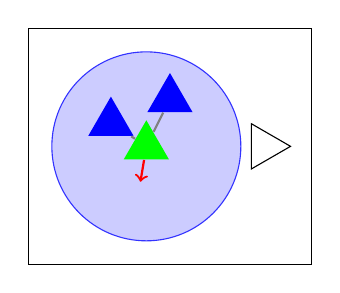
\begin{tikzpicture}[scale=0.6] % Adjust the scale as needed
            % Draw a semi-transparent blue circle with a dark border
            \draw[fill=blue!20, draw=blue!80] (0,0) circle (2);
            % Draw bounding box
            \draw (-2.5,-2.5) rectangle (3.5,2.5);
            % Define a triangle shape
            \node[regular polygon, regular polygon sides=3, minimum size=.5cm, fill,green] (t1) at (0,0) {};
            \node[regular polygon, regular polygon sides=3, minimum size=.5cm, fill,blue] (t2) at (.5, 1) {};
            \node[regular polygon, regular polygon sides=3, minimum size=.5cm, fill,blue] (t3) at (-.75, .5) {};

            % Outside, rotated
            \node[regular polygon, regular polygon sides=3, minimum size=.5cm, draw, rotate=30] (rotated) at (2.5,0) {};

            \draw[gray,thick] (t1) -- (t2);
            \draw[gray,thick] (t1) -- (t3);

            \draw[red,thick,->] (t1) -- (-.125,-.75);
        \end{tikzpicture}
        \caption{{\bf Collision avoidance (separation)}.}
    \end{subfigure}%
    \hspace{.5cm} % Adjust this value to increase or decrease the space
    \begin{subfigure}[t]{.28\textwidth}
        \centering
        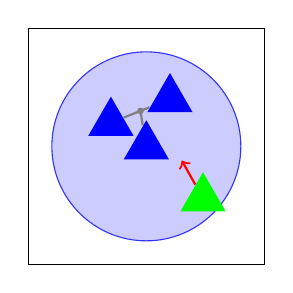
\begin{tikzpicture}[scale=0.6] % Adjust the scale as needed
            % Draw a semi-transparent blue circle with a dark border
            \draw[fill=blue!20, draw=blue!80] (0,0) circle (2);
            % Draw bounding box
            \draw (-2.5,-2.5) rectangle (2.5,2.5);
            % Define a triangle shape
            \node[regular polygon, regular polygon sides=3, minimum size=.5cm, fill,blue] (t1) at (0,0) {};
            \node[regular polygon, regular polygon sides=3, minimum size=.5cm, fill,blue] (t2) at (.5, 1) {};
            \node[regular polygon, regular polygon sides=3, minimum size=.5cm, fill,blue] (t3) at (-.75, .5) {};

            \node[regular polygon, regular polygon sides=3, minimum size=.5cm, fill,green] (t4) at (1.2, -1.1) {};

            \draw[gray, thick] (t1) -- (-.125,.75);
            \fill[gray, thick] (-.125,.75) circle (2pt);
            \draw[gray,thick] (t2) -- (t3);

            \draw[red,thick,->] (t4) -- (.75,-.3);
        \end{tikzpicture}
        \caption{{\bf Cohesion}: gravitate toward the center of the flock.}
    \end{subfigure}%
    \hspace{.5cm} % Adjust this value to increase or decrease the space
    \begin{subfigure}[t]{.28\textwidth}
        \centering
        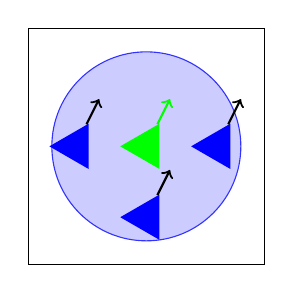
\begin{tikzpicture}[scale=0.6] % Adjust the scale as needed
            % Draw a semi-transparent blue circle with a dark border
            \draw[fill=blue!20, draw=blue!80] (0,0) circle (2);
            % Draw bounding box
            \draw (-2.5,-2.5) rectangle (2.5,2.5);
            % Define a triangle shape
            \node[regular polygon, regular polygon sides=3, minimum size=.5cm, fill,green,rotate=-30] (t1) at (0,0) {};
            \node[regular polygon, regular polygon sides=3, minimum size=.5cm, fill,blue,rotate=-30] (t2) at (-1.5, 0) {};
            \node[regular polygon, regular polygon sides=3, minimum size=.5cm, fill,blue,rotate=-30] (t3) at (1.5, 0) {};
            \node[regular polygon, regular polygon sides=3, minimum size=.5cm, fill,blue,rotate=-30] (t4) at (0, -1.5) {};

            \draw[green,thick,->] (t1) -- ++(.5, 1);
            \draw[black,thick,->] (t2) -- ++(.5, 1);
            \draw[black,thick,->] (t3) -- ++(.5, 1);
            \draw[black,thick,->] (t4) -- ++(.5, 1);
        \end{tikzpicture}
        \caption{{\bf Alignment}: maintain the same heading and speed.}
    \end{subfigure}
    \caption{The basic three rules of the Boids model. We show how the rules apply to a particular boid, marked
        green, and its neighbors, marked blue. Red arrows indicate the direction in which the observed boid has
        the tendency to move.}
    \label{fig:boids}
\end{figure}

\subsection*{Boids model implementation overview}

Each boid $B$ possesses three basic properties: position, velocity, and acceleration. Behavioral attributes include perception radius ($r_P$), separation radius ($r_S$), and perception angle ($fov$). The Euclidean distance, given by $d(p, q)^2 = (p_1-q_1)^2 + (p_2 - q_2)^2$, is utilized for distance computations.

The simulation loop updates boid directions based on three rules: \textbf{collision avoidance} (or \textbf{separation}), \textbf{alignment}, and \textbf{cohesion}. The avoidance direction is determined by summing the vector differences between the boid $B$ and its neighbors $B_i$ when their distance is within $r_S$. The cohesion direction is obtained by averaging the vector differences between the positions of boid $B$ and its neighbors $B_i$. The alignment direction is computed as the average velocity of neighboring boids $B_i$, subtracted from the velocity of the boid $B$, considering neighbors within a perception radius $r_P$.

The neighbors (all $B_i$) of a boid $B$ are determined using distance and angle conditions:
\begin{equation} \label{eq:neighbor_predicate}
    d(B, B_i)^2 < {r_P}^2 \, \land \, \text{AngleBetween}(B, B_i) \leq fov
\end{equation}
Modifying the base Boids model with the \textbf{field of vision} is an improvement inspired by \cite{JDemsar_predator_attacks}.

Additionally inspired by \cite{JDemsar_predator_attacks} is \textbf{occlusion}.
This effectively disregards boids that remain hidden from the view of a specific boid, as closer
boids obstruct their visibility (see Figure \ref{fig:occlusion}). Given a list of potential neighboring boids,
we must determine which are occluded and in turn take only the nearest (non-occluded) boids as neighbours. 
This is done by iterating through the list of neighboring boids of boid $B$ and computing the angle between all
neighbor pairs $(B_i, B_j)$. If the angle is below a threshold, boids $B_i$ and $B_j$ are considered occluded.
Then we just have to determine which neighbor is closer (which one blocks the other). This is done by computing
the minimum distance: $min(d(B, B_i), d(B, B_j))$. It is worth noting that we have only added occlusion
checks to the predator in our model.
\begin{figure}[h]
    \centering
    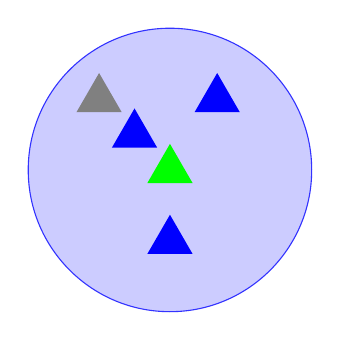
\begin{tikzpicture}[scale=0.6] % Adjust the scale as needed
        % Draw a semi-transparent blue circle with a dark border
        \draw[fill=blue!20, draw=blue!80] (0,0) circle (3);
		% Reference
        \node[regular polygon, regular polygon sides=3, minimum size=.5cm, fill,green] (boid1) at (0,0) {};
        % Occluded
        \node[regular polygon, regular polygon sides=3, minimum size=.5cm, fill,gray] (boid2) at (-1.5,1.5) {};
		% Neighbors
        \node[regular polygon, regular polygon sides=3, minimum size=.5cm, fill,blue] (boid3) at (-.75,.75) {};
        \node[regular polygon, regular polygon sides=3, minimum size=.5cm, fill,blue] (boid4) at (0,-1.5) {};
		\node[regular polygon, regular polygon sides=3, minimum size=.5cm, fill,blue] (boid5) at (1,1.5) {};
    \end{tikzpicture}
	\caption{Neighbors (blue) of the observed boid (green). Occluded boid is marked gray.}
	\label{fig:occlusion}
\end{figure}

In order to add even more realism, the \textbf{turn speed} of a boid is limited.
Whenever the acceleration of a boid is computed, the angle between the acceleration vector and the current heading vector is checked.
If it exceeds a threshold, the old heading is rotated by the maximum amount in the given direction and scaled by the magnitude of the acceleration.
Therefore boids have a maximum value in which they can turn at each step of the simulation.

\subsection*{Escape maneuvers}

In the HoPE model, which was proposed in \cite{papadopoulou2022emergence} and that we have tried to
reproduce, discrete escape maneuvers are introduced. These maneuvers involve individual turns away from
the predator's heading, with turning angles and durations drawn from gamma distributions tailored to empirical
data. Each flock member's likelihood of maneuvering is determined by a unique baseline escape tendency and
proximity to the predator. During maneuvers, coordination with neighbors is absent. Additionally, basic Boids
rules guide prey away from the predator, while in non-maneuvering states.

We have implemented three escape maneuvers: \textbf{position-based}, \textbf{direction-based}, and \textbf{zig-zag}
escape maneuvers. Due to \textit{separation} embedded in our model, in the position-based escape maneuver, prey moves
away from the predator once it gets too close. In the direction-based escape behavior, we simply compute the angle
between the heading of the predator and prey. We take the sign of this angle and rotate the heading of the prey by
$+$ or $-$ 90°, depending on the sign. The zig-zag escape maneuver simply alternates the prey direction in fixed
time intervals. Some of these maneuvers result in patterns shown in Figure \ref{fig:escape_maneuvers}.
\begin{figure}[h]
	\centering
	\begin{subfigure}[t]{.45\textwidth}
		\centering
		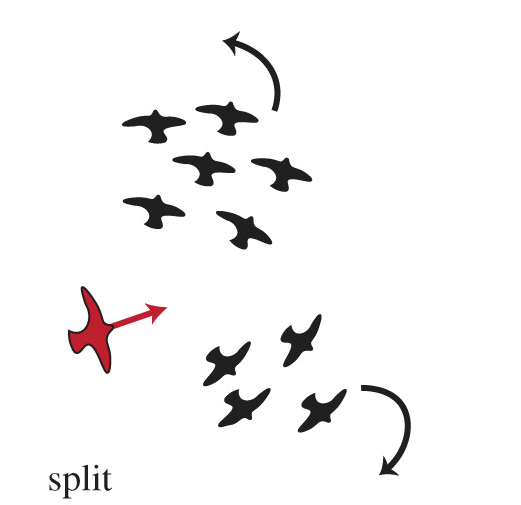
\includegraphics[width=0.6\linewidth]{article_split.png}
	\end{subfigure}%
	\hspace{.5cm} % Adjust this value to increase or decrease the space
	\begin{subfigure}[t]{.45\textwidth}
		\centering
		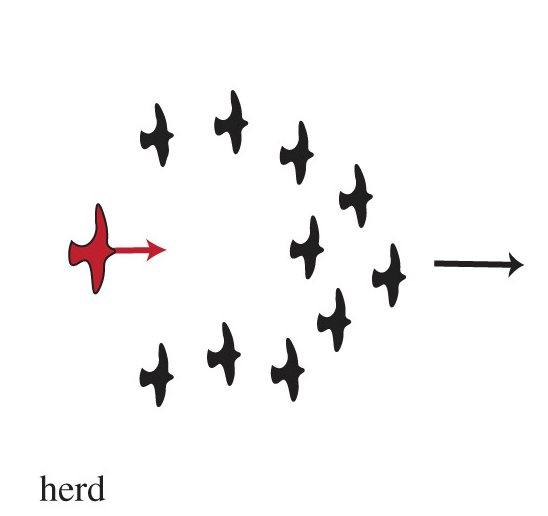
\includegraphics[width=0.6\linewidth]{article_herd.png}
	\end{subfigure}
	\caption{The patterns emerging from position-based (left picture) and direction-based (right picture) escape maneuvers.}
	\label{fig:escape_maneuvers}
\end{figure}

\subsection*{Predators}

We have implemented four predator attack strategies, with three detailed and simulated in \cite{JDemsar_predator_attacks}.
The first targets the flock's center,
the second goes for the closest prey,
and the third selects the most isolated prey.
In the last strategy, the predator simply attacks a random target.
\section*{Results}

In Figure \ref{fig:sim_split}, we demonstrate the split escape maneuver modeled by our simulation.
\begin{figure}[h]
    \centering
    \begin{subfigure}[t]{0.3\linewidth}
        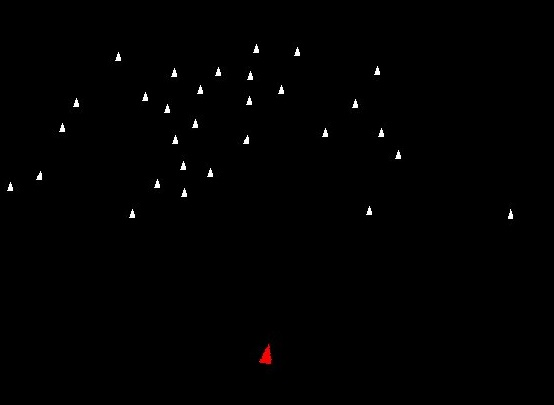
\includegraphics[width=\linewidth]{boids_step_146.jpg}
        \caption{Predator chasing a group of boids (step $146$).}
    \end{subfigure}%
    \hspace{0.02\linewidth} % Adjust this value to increase or decrease the space
    \begin{subfigure}[t]{0.3\linewidth}
        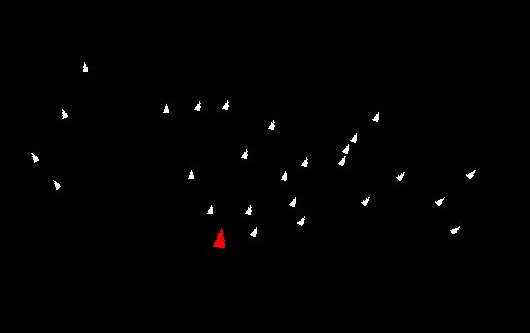
\includegraphics[width=\linewidth]{boids_step_233.jpg}
        \caption{Start of split pattern (step $233$).}
    \end{subfigure}%
    \hspace{0.02\linewidth} % Adjust this value to increase or decrease the space
    \begin{subfigure}[t]{0.3\linewidth}
        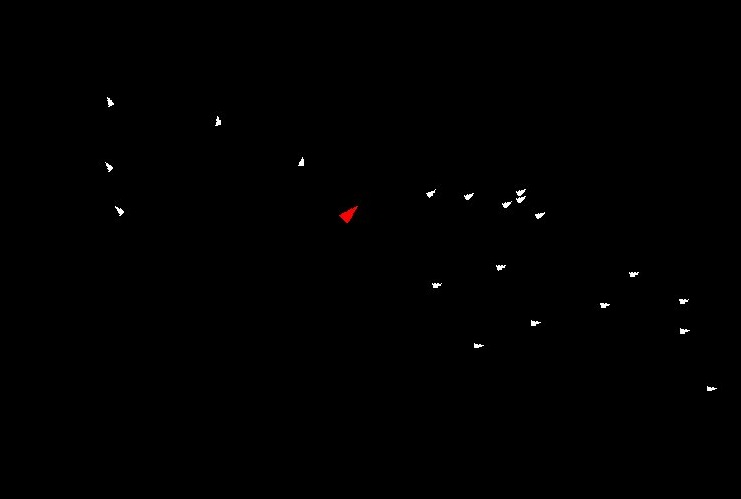
\includegraphics[width=\linewidth]{boids_step_261.jpg}
        \caption{Predator caught a prey, split continues (step $261$).}
    \end{subfigure}
    \caption{A demonstration of the split escape maneuver. Predator and prey positions
	are shown at various steps of a simulation.}
	\label{fig:sim_split}
\end{figure}


\pagebreak

\section*{Discussion}

This concludes boids implementation with additional realsitic features.
The simulation itself was heavily parameterized aswell, making tweakings easiser and more reproducible.

There is still room for improvement in the visualization of the simulation (add traces, add predators target, ...).

The most important aspect which remains is the implementation of different escape manuevers and predator tactics and the comparisons of the latter.

\acknow{Matija Ojo: Add realistic features, fix escape manuevers, report, Miha Krajnc: Escape manuevers, Janez Kuhar: report, Marko Adžaga: Researching sources and report}

\showacknow % Display the acknowledgments section

% \pnasbreak splits and balances the columns before the references.
% If you see unexpected formatting errors, try commenting out this line
% as it can run into problems with floats and footnotes on the final page.
%\pnasbreak

\begin{multicols}{2}
    \section*{\bibname}
    % Bibliography
    \bibliography{bibliography}
\end{multicols}

\end{document}